Pulsars are highly magnetised neutron stars which have a hot emitting
region on their surface which produces a beam of electromagnetic
radiation. As the neutron star rotates its beam sweeps out across
space, and we see it as a brief, frequent flash, much like a
lighthouse beam.

Pulsars were discovered, accidentally, in 1967 by Jocelyn Bell under
the supervision of Anthony Hewish, while investigating fluctuations in
the flux densities of extragalactic radio galaxies and quasars. This
interplanetary scintillation is caused by the passage of radio waves
through the solar wind, and depend on the angular size of the source,
and promised to give a measure of the cosmological distribution of
radio galaxies, constraining models of galaxy formation.

\section{Early deductions}
\label{sec:early-deductions}

The pulses from the first pulsars to be detected showed no parallax
effects, but did show timing variations due to the Earth's orbit,
hence were far outside the solar system. They sweep through the radio
band, implying that they have been dispersed by the ISM. The amount of
dispersion implies that they are local galactic objects. Their signals
are bright ($\sim 20\,\text{Jy}$), and these vary in strength. The
pulses have a length shorter than $0.016\,\second$, implying a
diameter around $5\,000\,\kilo\meter$.

\section{Derived properties}
\label{sec:derived-properties}

\subsection{Brightness temperature}
\label{sec:brightn-temp}

The brightness temperature of an object is the temperature which
observing the object would produce in an antenna, and is defined
\begin{equation}
  \label{eq:89}
  T~b = \frac{B c^2}{2 \nu^2 k~B}
\end{equation}
for $B$ the brightness, $c$ the speed of light, $\nu$ the frequency of
the radiation, and $k~B$ the Boltzmann constant.

\begin{example}[Brightness temperature of CP1919]
  We assume a distance of $1\,\kilo\text{pc}$ and a diameter of
  $10\,\kilo\meter$, then the solid angle of the source is
\[ \Omega~s \approx \pi \qty( \frac{5\,\kilo\meter}{3\e{16}\,\kilo\meter} ) = 8\e{-32}\,\steradian \]
and the brightness is
\[ B = \frac{S}{\Omega~S} = \frac{20\e{-26}\,\watt\,\meter^{-2}\,\hertz^{-1}}{8\e{-32}\,\steradian} \]
Then
\[ T~b = 10^{30}\,\kelvin \]
\end{example}
Note, the limit on brightness temperature from synchrotron radiation is around $10^{12}\,\kelvin$.

\subsection{Density}
\label{sec:density}

The density of a pulsar can be inferred from the centrifugal force
which its rotation period implies.  Consider the fastest known pulsar,
PSR\,J1748--2446ad, which is in the globular cluster Terzan 5.

\begin{example}[The density of PSR\,J1748--2446ad]
  This pulsar rotates at a rate $\nu = 716\,\hertz$. Using the mass,
  $M$, the radius, $R$, and the rotation rate $\omega = 2 \pi / P$,
  centrifugal breakup occurs if
\[ \omega^2 R > \frac{GM}{R^2} \]
and so, if 
\[ P^2 < \frac{4 \pi R^3}{3} \frac{3 \pi}{GM} \] then the mean
density, $\rho$, is constrained to be \[\rho > \frac{3 \pi}{GP^2} =
7\e{16}\,\kilo\gram\,\meter^{-3} \]
\end{example}

\subsection{Size}
\label{sec:size}

Assuming that the mass of a neutron star is $1.4\,M_{\odot}$, from
this density, the radius must be less than $21\,\kilo\meter$.

\subsection{Magnetic field}
\label{sec:magnetic-field}

Neutron stars have strong magnetic fields; simple arguments based
around the conservation of magnetic flux during the collapse of the
progenitor star suggests $B \sim 10^8\,\tesla$, but more sophisticated
arguments imply $10^9$ to $10^{11}\,\telsa$. Taking the pulsar to be a
rapidly rotating bar magnet, we have radiation emission as if from a
dipole, with luminosity
\begin{equation}
  \label{eq:90}
  L = \frac{\mu_0 \abs{\ddot{m}}^2 \sin[2](\theta)}{6 \pi c^3} = \frac{2 \pi R^6 B~P^2 \omega^4 \sin[2](\theta)}{3 c^3 \mu_0}
\end{equation}
where $B~P$ is the magnetic flux density of the pulsar at the pole,
and $R$ is its radius. These waves are the primary source of radiation
loss, but do not produce the radiation seen in radio. They are below
the local plasma frequency, so are not transmitted away from the
nebula around the pulsar.

\subsection{Radiation braking}
\label{sec:radiation-braking}

The only source of energy for the pulsar is the rotational kinetic
energy of the rotation about the pulsar's axis, about which the moment
of inertia, $I_{zz}$ produces energy
\begin{equation}
  \label{eq:91}
  E = \half I_{zz} \omega^2
\end{equation}
and so
\begin{equation}
  \label{eq:92}
  L = - \dot{E} = - I_{zz} \omega \dot{\omega}
\end{equation}
Thus, radiation brakes the pulsar, so
\begin{equation}
  \label{eq:93}
  \dot{\omega} = - \frac{2 \pi R^6 B~P^2 \sin[2](\theta)}{3 c^3 \mu_0 I_{zz}} \omega^3
\end{equation}
Such a pulsar has a braking index of $n=3$, where the braking index is
defined from the relation
\begin{equation}
  \label{eq:94}
  \dot{\omega} \propto -\omega^n
\end{equation}
The minimum magnetic field can be determined from this and knowledge
of the spin-down rate, 
\[ B~{min} = 3.2\e{15} \qty( P \dot{P} )^{\half}\,\tesla \]

\begin{figure*}
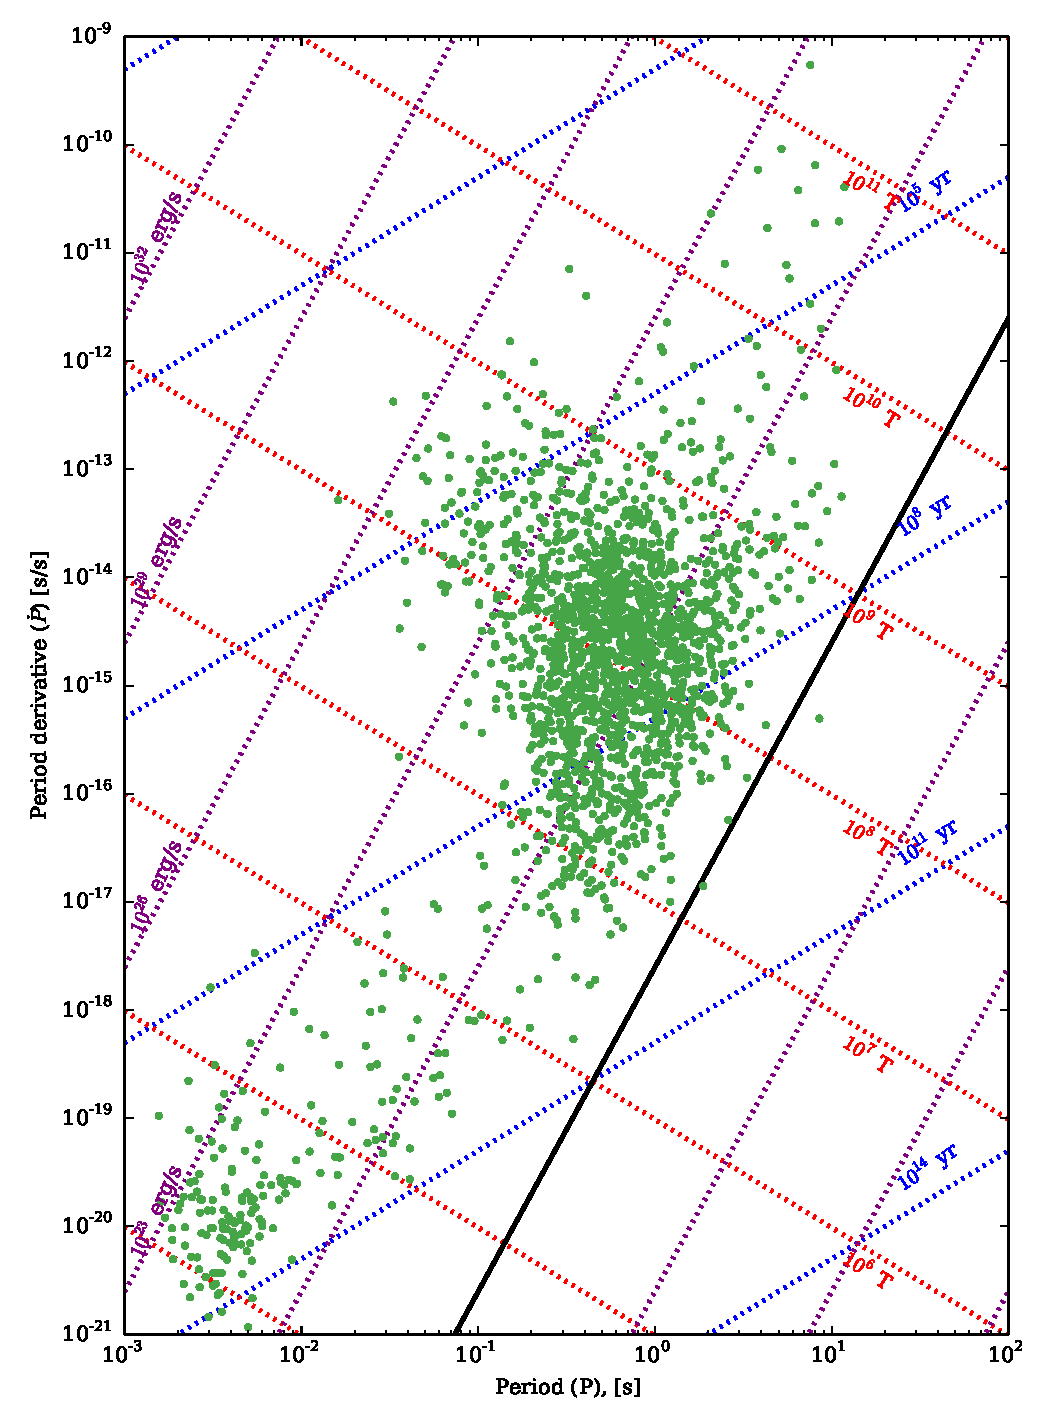
\includegraphics{figures/ppdot.pdf}
\caption{The $P$-$\dot{P}$ diagram of all of the known pulsars, with characteristic ages marked in green.}
\label{fig:ppdot}
\end{figure*}

\subsection{Spin-down Luminosity}
\label{sec:spin-down-luminosity}



\subsection{Characteristic age}
\label{sec:characteristic-age}

The characteristic age of a pulsar is an approximation of the age of a
pulsar assuming that it had an initial period smaller than the current
one, has no magnetic field decay, and a braking index of $n=3$. From
this we define the characteristic age, $\tau$, as
\begin{equation}
  \label{eq:95}
  \tau = \frac{P}{2 \dot{P}}
\end{equation}
Allowing for an explicit $n$,
\begin{equation}
  \label{eq:96}
  \tau = \frac{P}{(n-1) \dot{P}} \qty[ 1 - \qty(\frac{P_0}{P})^{n-1} ]
\end{equation}
for $P_0$ the initial spin period, and $\dot{P}_0$ the initial spin
period derivative.

\subsection{Timing stability}
\label{sec:timing-stability}

The stability of some pulsars' rotation periods rivals that of atomic
clocks over long time periods ($\sim 1\,\text{yr}$), once relative
motion and a constant spin-down rate. At some level all pulsars show
\emph{timing noise}; these may be due to gravitational effects along
the propagation of the wave through space.

\subsection{Astrometric position}
\label{sec:astrometric-position}

Pulsar signals must be Doppler corrected for the relative motion of
the pulsar and the Earth; this correction is sensitive to the position
of the pulsar in the sky. The angular resolution of observations of a
pulsar are equivalent to those of an aperture of radius
$1\,\text{AU}$. Then for a $100\,\hertz$ pulsar,
\[\theta \approx \frac{\lambda}{D} = \frac{c/\nu}{2\,\text{AU}} \approx 2\,\text{as}\]
We can, however measure over many cycles, and so
\[ \theta = \frac{d}{D} = \frac{c \Delta \tau}{2\,\text{AU}} \approx
206 \Delta \tau\,\text{as} \] with the best timing resolutions $\Delta
\tau \approx 50\,\nano\second$, and hence astrometric precisions of
$\theta \approx 10\,\micro\text{as}$.

\subsection{Gravitational physics}
\label{sec:grav-phys}

Binary neutron star systems have two orbiting masses which form a
rotating mass quadrupole, and generate gravitational waves with a
luminosity of
\begin{equation}
  \label{eq:97}
  L~G = \frac{32}{5} \frac{G^4}{c^5} \frac{m_1^2 m_2^2 (m_1+m_2)}{a^5}
\end{equation}
at twice the orbital frequency.

By monitoring the travel times of pulses it is possible to infer the
presence of a gravitational wave. Say a pulse is sent at $(x_1,t_1)$,
and the strain along the line of sight is $h$, then the fractional
change in the arrival rate can be reduced to the difference in the
strain at the start and the end of the transmission,
\begin{equation}
  \label{eq:98}
  \frac{\var{\nu}}{\nu} = h(x_1,t_1) - h(x_2, t_2) 
\end{equation}
This is the only know way to detect very low frequency gravitational
waves, producing a timing residual of
\begin{equation}
  \label{eq:99}
  R(t) = - \int_0^t \frac{\var{\nu}}{\nu} \dd{t}
\end{equation}

\subsection{Equation of state}
\label{sec:equation-state}

Variations in the rotation of pulsars allow the equation of state to
be inferred. The density profile determines the moment of inertia,
\[ I_{zz} = kMR^2 \] for $k=2/5$ for a uniform ball. Glitches indicate
that there is a superfluid internal structure which couples to the
crust, creating steep rotation-rate gradients , deforming the crust.

\subsection{Extreme plasmas}
\label{sec:extreme-plasmas}

Pulsars are a complex problem in relativistic plasma physics, as
neither the radiation mechanism nor the structure of the magnetosphere
is well understood. The plasma of the magnetosphere forms a pulsar
wind nebula, and these are visible in x-ray wavelengths for the crab
and vela pulsars. The double pulsar system, PSR\,J0737-3039, provides
the most sensitive measurements of these nebula, as the pulsar beams
from the two components pass through the other's wind nebula
frequently.

\subsection{Extrasolar planets}
\label{sec:extrasolar-planets}

Periodicities in the timing residuals of PSR\,B1257+12 are consistent
with the gravitational effects of four planets.


%%% Local Variables: 
%%% mode: latex
%%% TeX-master: "../project"
%%% End: 
